\section*{Problem Sheet 3}
\label{sec:ps2}
\newcounter{psFourQuestions}
\setcounter{psFourQuestions}{0}
\renewcommand{\NewQuestion}[1]{\stepcounter{psFourQuestions}\subsection*{Exercise \arabic{psFourQuestions}: #1}}


\NewQuestion{Mixing}
\begin{enumerate}[a)]
 \item Draw Feynman diagrams that mediate mixing in \prt{K^0}, \Do,
  \Bdo\ and \Bso\ mesons. 
%%
 \answerbox{
  \begin{tabular}{cccc}
   \prt{K^0} & \Do & \Bdo & \Bso \\
   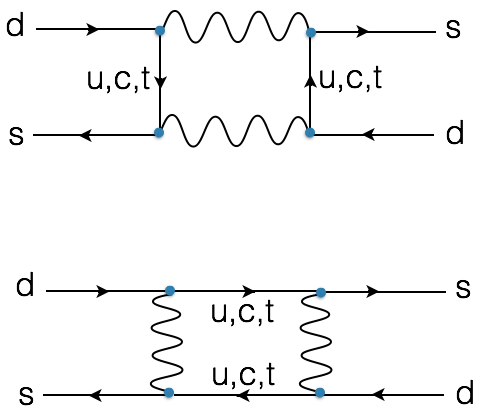
\includegraphics[width=0.22\textwidth]{problemsheets/ps4figs/KaonMixing} &
   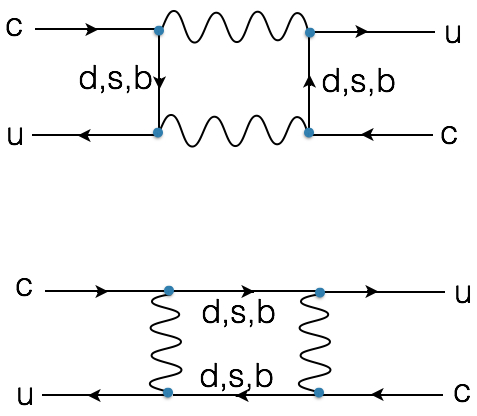
\includegraphics[width=0.22\textwidth]{problemsheets/ps4figs/DMixing} &
   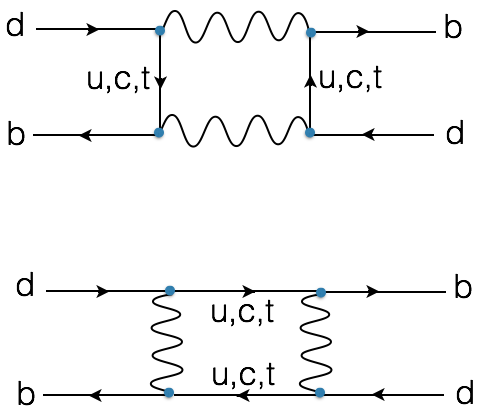
\includegraphics[width=0.22\textwidth]{problemsheets/ps4figs/BdMixing} &
   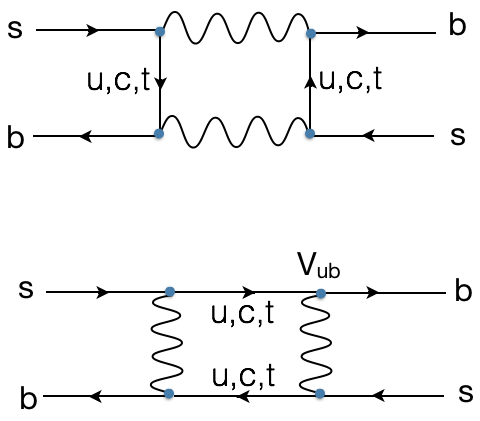
\includegraphics[width=0.22\textwidth]{problemsheets/ps4figs/BsMixing}
   \end{tabular}
   \\ (Above the $W$ is indicated by a wavey line (like a photon - given electroweak unification, that actually makes some sense); the other convention, more often used in this course than the wavey line, is to draw it as a broken line, $----$).
 }
\item Give an estimate of $\frac{\Delta m_d}{\Delta m_s}$, where $\Delta m_d$ is
  the mass difference between the mass eigenstates in the \Bdo\ system
  and $\Delta m_s$ is the equivalent quantity for the \Bso\ system. Hint: $\Delta m$ is proportional to the mixing frequency,
  which in turn is proportional to the magnitude of the mixing Feynman
  diagram.
%%
  \answerbox{ To answer this, we use that the \Bdo\ and \Bso\ mixing
    amplitude is completely dominated by the diagrams with an
    internal top quark line\\
    \begin{tabular}{cc}
      \Bdo & \Bso \\
      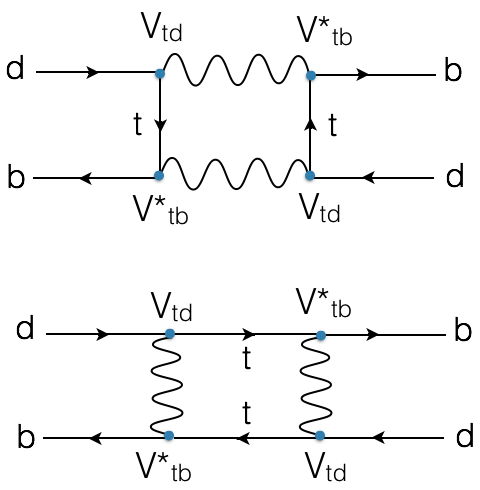
\includegraphics[width=0.33\textwidth]{problemsheets/ps4figs/BdMixingWithCKM} &
      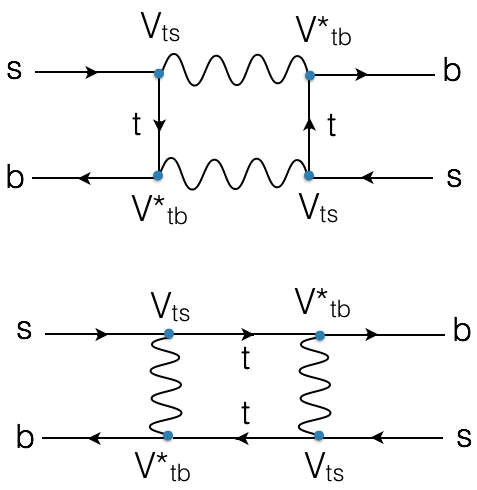
\includegraphics[width=0.33\textwidth]{problemsheets/ps4figs/BsMixingWithCKM}
    \end{tabular}\\
    (NOTE: the wiggly lines in the above diagrams are W, not photons.)\\
    The ratio of the mass differences should
    be approximately the ratio magnitude of these diagrams. And the
    magnitude of each diagram is proportional to the product of the
    relevant CKM matrix elements. So we get:
    \[
    \frac{\Delta m_d}{\Delta m_s} \approx \left| \frac{(V_{td}
        V_{tb}^*)^2}{(V_{ts} V_{tb}^*)^2} \right| = 
    \left| \frac{(V_{td})^2}{(V_{ts})^2} \right| = {\color{red}\left(\frac{0.0087}{0.041}\right)^2 
    \approx 0.045}
    \]
}
\item Why is the mixing frequency in the charm system the lowest of them all?
\answerbox{The GIM mechanism works much better in charm than in B and K. If all quark masses were the same, all FCNC would cancel exactly. However, the top quark is much heavier than all other quarks and breaks the GIM mechanism quite badly in B and K FCNC. I charm FCNC (like the mixing diagram, but also other FCNC), the internal quarks are $d, s, b$. Their masses are much closer together ($b$ has a mass of \un{4.2}{GeV}, compared to top with \un{173}{GeV}). For this reason, GIM cancellation of FCNC works much better in charm. In addition, the couplings between the $c, u$ quarks and the $b$ are quite small (while in the B system, $V_{tb}$ is quite large, further enhancing the GIM-destroying top contribution).

A more mathematical solution would have used that the size of the contribution from each internal quark line is proportional to its mass, but this level of detail was not required for this question.
}
\end{enumerate}

\NewQuestion{CP violation in the interference between mixing and decay}
\begin{enumerate}
\item Draw the tree diagram for \prt{\Bdo \to \pi^+ \pi^-}
\answerbox{
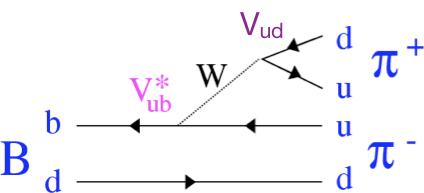
\includegraphics[width=0.45\textwidth]{problemsheets/fig/B2pipiTree.png}
}
\item Considering only the mixing diagram and this tree diagram, what \cp-violating phase would be measured in the time-dependent decay rate asymmetry \prt{\Bo \to \pi^+\pi^-}?
\answerbox{ The two interfering decay path are 
  \begin{enumerate}[1]
  \item \prt{\Bdo \to \pi^+ \pi^-}
  \item \prt{\Bdo \to \Bdob \to \pi^+ \pi^-}
  \end{enumerate}
  Their phases:
  \begin{itemize}
  \item \prt{\Bdo \to \pi^+ \pi^- } is proportional to $V_{ud}V_{ub}^*$ and has therefore weak phase $\gamma$ (from $V_{ub}^*$). It also might have a strong phase $\delta$, so the total phase is $\gamma + \delta$.
  \item \prt{\Bdo \to \Bob} is proportional to $V_{tb}^{*2} V_{td}^2$ which has phase $-2\beta$. (There are no meaningful strong phases in these mixing diagrams.)
  \item \prt{\Bdob \to \pi^+ \pi^-} is the CP-conjugate to \prt{\Bdo \to \pi^+ \pi^- }, so it must have the opposite weak phase and the same strong phase: -$\gamma + \delta$
  \end{itemize}
  The phase difference between the path is therefore 
  $2\beta + 2\gamma$.
}
\item Draw the penguin diagram for \prt{\Bdo \to \pi^+ \pi^-}
\answerbox{
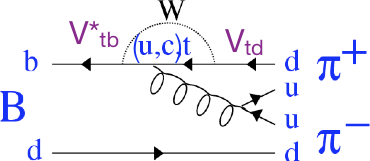
\includegraphics[width=0.45\textwidth]{problemsheets/fig/B2pipiPeng.png}
}
\item Why is the presence of the penguin diagram in this case a considerably worse nuisance than in $\Bdo \to J/\psi K_S$?
\answerbox{In the case of \prt{\Bdo \to J/\psi K_S}, tree and penguin had the same phase. Here they do not (the dominant contribution of the penguin diagram, with the internal top quark, has no phase, while the tree contribution has phase $-\gamma$). Therefore in order to calculate the total phase we need to know the relative magnitude of these diagrams. This is a major headache, because the strong interaction plays an important role, here, and makes this difficult to calculate. For this reason, phases measured in \prt{\Bdo \to \pi^+ \pi^-} are really difficult to relate to CKM phases (and thus SM predictions).}
\item Why can \prt{B_d \to K^{*0}\overline{K}^{*0}} not proceed via a tree diagram?
\answerbox{Looking at the quark content, we start off with only down-type quarks ($\overline{b}, d$) and end with a different set of down-type quarks ($s\overline{d}, \overline{s}d$), hence we need a flavour changing neutral current.}
\item Draw the penguin diagram for \prt{B_d \to K^{*0}\overline{K}^{*0}}
\answerbox{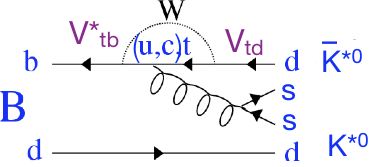
\includegraphics[width=0.5\textwidth]{problemsheets/fig/B02KstarKstar}}
\item Which additional complication will arise in the CP violation measurement with \prt{B_d \to K^{*0}\overline{K}^{*0}}, given that the final state has two spin-1 particles?
\answerbox{Two spin one particles can combine to total spin $S=|S_1 - S_2|, |S_1 - S_2|+1, \cdots S_1 + S_2$. In this case the options are $0, 1, 2$. The initial state as spin zero. To form a total $\vec{L} + \vec{S}$ of zero, the final state particles have three options, $S=2, L=2$, $S=1, L=1$ and $S=0, L=0$. These correspond to different CP eigenvalues of the final state. The measurement still works, as these CP eigenstates can be disentangled by considering the angular distribution of the decay products, but it's a significant complication in the analysis.}
\end{enumerate}

\NewQuestion{The phase of $V_{ts}$}
According to our formula sheet, $V_{ts}$ is real. However, it does have a very small complex phase, $V_{ts} = -|V_{ts}|e^{-i\beta_s}$. Propose a way of measuring that phase. To simplify things, if there is both a penguin and a tree contribution, you can ignore the penguin contribution.
\answerbox{There are of course many possible answers. This one seems to me the most obvious one, but you might have found an even better one.

Clearly, you want to use \prt{B_s} mesons, as they have an $s$ quark. $V_{ts}$ shows up in the \prt{B_s \to \overline{B}_s} mixing diagram in the same way as $V_{td}$ does in the \prt{B_d \overline{B}_d} mixing diagram. Simply replacing all $d$ quarks with $s$ quarks in \prt{\Bdo \to J/\psi K_S} gets you to the decay \prt{\Bdo \to J/\psi \phi}, as a good candidate. The relevant diagrams are the mixing diagrams that laready featured in the previous question\\
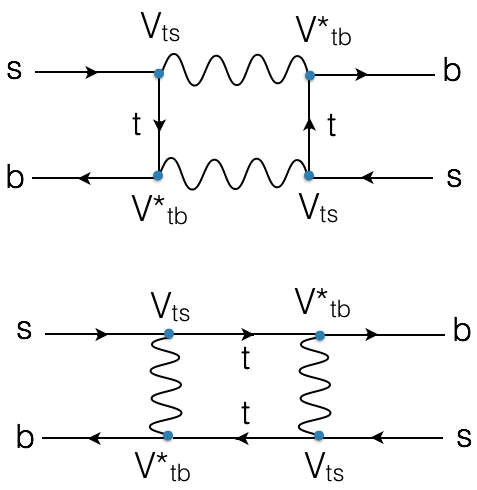
\includegraphics[width=0.3\textwidth]{problemsheets/ps4figs/BsMixingWithCKM}\\
both proportional to $(V_{ts} V_{tb}^*)^2$
and the decay diagrams.(NOTE: the wiggly lines in the above diagrams are W, not photons.)\\
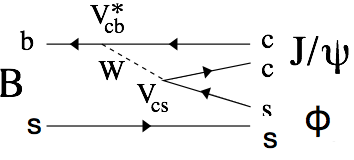
\includegraphics[width=0.3\textwidth]{problemsheets/fig/Bs2JpsiPhiTree}
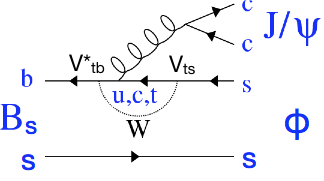
\includegraphics[width=0.3\textwidth]{problemsheets/fig/Bs2JpsiPhiPeng}\\
where the 2nd one is a penguin diagram. Intriguingly, it is sensitive to exactly the $V_{ts}$ we are interested in, but we were told to ignore penguins, so we do. Then
\begin{itemize}
\item $\prt{B_s \to J/\psi \phi} \propto e^{i0}$
\item $\prt{B_s \to \overline{B}_s} \propto e^{-i 2 \beta_s}$
\item $\prt{\overline{B}_s \to J/\psi \phi} \propto e^{i0}$
\end{itemize}
where we ignored strong phases, knowing that they cancel in decays to CP eigenstates. So the total phase difference is $2\beta_s$. Note that in reality, this is one of the most interesting measurements, because $\beta_s$ is really quite small and also very precisely predicted in the SM (through the unitarity of the CKM matrix and other measurements), and new physics in either the penguin or the mixing diagram could significantly affect the measured phase.
}

\NewQuestion{Rare Decays}
Estimate the decay rate ratio
\[
R_{B} = \frac{\Gamma(\prt{D^0 \to \mu^+\mu^-})}{\Gamma(\prt{D^0 \to e^+e^-})}
\]
\answerbox{
The coupling constants involved in this are identical (lepton universality). The only difference is in the masses of the particles. The \prt{D^0} is a spin 0 particle, the decay products are two spin $\half$ particles. This means that one of the must have the "wrong" helicity (while the other can have the right one).
In the lecture notes we find 
\begin{align*}
P(\mathrm{"wrong" chirality}) &\approx 
 \half \left(1 - \beta \right)
 =
 \frac{m^2}{ 2E^2 \left( 1 + \frac{|\vec{p}|}{E}\right)}
\end{align*}

Now $E$ is in both cases the same, it's got to be $\half m_D$. Let's calculate $|\vec{p}|$.
\begin{align*}
 \vec{p}_{\mu} & = \sqrt{E^2 - m_{\mu}^2}
 \\ &= \sqrt{\frac{1}{4} m_D^2 - m_{\mu}^2}
 \\ &= \sqrt{\frac{1}{4} \left((1900)^2- (106)^2\right)} \mathsf{MeV}
 \\ &= \un{944}{MeV} \approx \half m_D
\end{align*}
Similarly
\begin{align*}
 \vec{p}_{e} & = \sqrt{E^2 - m_{e}^2}
 \\ &= \sqrt{\frac{1}{4} \left((1900)^2- (0.5)^2\right)} \mathsf{MeV}
 \\ &= \un{949}{MeV} \approx \half m_D
\end{align*}
So the two are essentially the same. The reason for this is that the \prt{D^0} mass is much larger than the $\mu^+ \mu^-$ as well as the $e^+ e^-$ mass.

From the above we also see that the phase space factor ($\propto |\vec{p}|$) is essentially the same for the two modes.

Now what we really need to calculate is that one lepton has the right helicity, and the other the wrong one, we have
\begin{align*}
    P(\mathrm{one\,right\,one\,wrong})
    &=\left( \frac{m^2}{ 2E^2 \left( 1 + \frac{|\vec{p}|}{E}\right)}\right)
    \cdot 
    \left(1 - \frac{m^2}{ 2E^2 \left( 1 + \frac{|\vec{p}|}{E}\right)}\right)
\end{align*}
But that 2nd factor is so close to $1$ that it's not really worth including. In an exam you would not be expected to. Here, for fun, I calculate it for the $\mu$:
\[
\left(1 - \frac{m_{\mu}^2}{ 2E^2 \left( 1 + \frac{|\vec{p}|}{E}\right)}\right)
\approx
\left(1 - \frac{m_{\mu}^2}{m_D^2}\right)
=0.997
\]
So indeed, we can ignore it. With this, we get for the ratio
\[
R_{B} = \frac{\Gamma(\prt{D^0 \to \mu^+\mu^-})}{\Gamma(\prt{D^0 \to e^+e^-})}
\approx \frac{m_{\mu}^2}{m_{e}^2}
\sim 44,000
\]
PS: In an exam situation, a sentence like "The \prt{D^0} mass is much bigger than either $\mu^+\mu^-$ or $e^+ e^-$, therefore we can assume $E\approx |\vec{p}|$" instead of calculating $|\vec{p}|$ would have sufficed. Also, to justify ignoring phase space,
"The D mass is much bigger than either $\mu^+\mu^-$ or $e^+ e^-$, therefore the phase-space factor in the two cases will be the same" would have been fine.
}
\NewQuestion{Conservation laws.}
For each of the following decays, state if the decay
allowed or forbidden. If the decay is forbidden, state all
conservation laws that are violated. If it is allowed, state, with
reasons, which force is predominantly responsible.
\\
In all cases, we are considering the decays of free particles (in
contrast, for example, to protons or neutrons bound inside a nucleus).
\begin{enumerate}
\setlength{\itemsep}{0ex}
  \item $D^{*+} \to D^0 \pi^+$ 
  % 
  \answerbox{2 pt allowed - no conservation laws will prevent this
    from proceeding via the strong interaction, so that will
    dominate.  }
  \item $\tau^- \to e^- \gamma$
  \answerbox{
    1pt
    forbidden, violates charged lepton flavour conservation
  }
  \item $J/\psi \to \mu^+ \mu^-$
  \answerbox{Allowed, QED ($\mu^+ \mu^-$ have no colour charge)}
  \item $p \to \overline{n} e^+ \overline{\nu}_{e}$ 
  \answerbox{
    Forbidden, since it violates
    \begin{itemize}
    \item Energy conservation ($m_n > m_p$)
    \item Baryon number conservation ($B_p = +1, B_{\overline{n}} = -1$)
    \item Lepton number conservation ($L({p}) = 0, L(e^+) = -1, L(\overline{\nu_e}) = -1$)
    \item (it also violates lepton flavour, but this is implied in the above).
    \end{itemize}
  }
  \item $\pi^0 \to \gamma\gamma$
  \answerbox{ allowed, electromagnetic (because of photons)}
  \item $\gamma \to e^+ e^-$
  \answerbox{
     forbidden, energy and momentum conservation
     (as an aside, note that photons that hit something heavy, like a nucleus, can convert to $e^+ e^-$, the nuclear recoil then takes care of momentum conservation)
   }
  \item $\mu^- \to e^- \overline{\nu}_{e} \nu_{\mu}$
  \answerbox{
    allowed, has to be a weak decay due to lepton flavour change
  }
\item $f_0(980) \to \pi^+\pi^-$
  \answerbox{
    can decay strongly, so it will
  }
  \item $f_0(980) \to \pi^+\pi^-\pi^0$
  \answerbox{
    This processes violates parity as the parity of the 3pi system is -1 (see the example in your notes). As this processes cannot occur through the weak force, it is forbidden.  
  }
  %%
\item $\rho \to \pi^0 \eta^0$
  \answerbox{Violates $C$ (charge conjugation) symmetry. 
  So if this decay is possible at all, it has to proceed via the weak interaction.
    (Note that it also violates strong isospin.)
  }
  \item $p \to \pi^+ \pi^0$
  \answerbox{Absolutely forbidden: violates baryon number conservation}
  \end{enumerate}
\NewQuestion{Strong interaction}
Which of these decays is allowed by the strong interaction?
(here, as well as in the exam, please assume that isospin is a good symmetry of the strong interaction)
\begin{enumerate}
  \item $\rho \to \pi^+ \pi^-$
  \answerbox{allowed}
  \item $\Omega^- \to \Lambda \pi^+$
  \answerbox{$sss \to uds  u\bar{d}$ violates flavour conservation. Also violates isospin}
  \item $\Upsilon(4S) \to \Lambda_c \overline{\Sigma}_c^-$
  \answerbox{violates isospin}
  \item $\Sigma_c^+ \to p \overline{D}^0$
  \answerbox{violates isospin}
\end{enumerate}
